
\documentclass[12pt]{article}
\usepackage[english]{babel}
\usepackage[utf8x]{inputenc}
\usepackage{amsmath}
\usepackage[table,xcdraw]{xcolor}
\usepackage[colorinlistoftodos]{todonotes}
\graphicspath{ {./images/} }
\usepackage{algpseudocode}
\begin{document}

\begin{titlepage}
\newcommand{\HRule}{\rule{\linewidth}{0.5mm}}
\center
\HRule \\[.8cm]
{ \huge \bfseries Homework Assignment}\\[0.4cm]
\HRule \\[1cm]
\begin{center} 
04 June 2022
\end{center} 

\centering
\begin{minipage}{\textwidth}
\begin{flushleft} \large
\vspace{10cm}
\emph{Name: Dumitrescu Marian-Daniel }\\
\emph{Speciality: Calculatoare Română 2nd Year}\\
\emph{Group: 2.2 A}\\
\end{flushleft}
\end{minipage}

\vfill

\end{titlepage}

\section{Problem statement}
\hspace{0.5cm} Let us suppose the k × k grid presented in Figure 2. The grid is configured with a pattern of walls. You are required to place n archers on this grid such that they cannot shoot each other. An archer can shoot up, down, left, right and also diagonally and its shoot can reach at most w locations in all directions, up to the grid edges.\\

For this problem we will need to input this data: the length of the grid: \textbf{k}; the number of archers: \textbf{n}; the strength(attack range) of the archers: \textbf{w}; and finally the initial grid. The walls are also part of the archer's grid and their position does not change. The final position of the archers must be determined so that they will not attack each other.\\

We will consider some examples to see how the problem should be resolved:\\
\begin{itemize}
    \item Example 1: 
\begin{tabular}{|cccc|c|cccc|}
\hline
\multicolumn{4}{|c|}{Input}                                                   &  & \multicolumn{4}{c|}{Output}                                                  \\ \hline
\multicolumn{1}{|c|}{k} & \multicolumn{1}{c|}{}  & \multicolumn{1}{c|}{4} &   &  & \multicolumn{1}{c|}{}  & \multicolumn{1}{c|}{}  & \multicolumn{1}{c|}{}  &   \\ \hline
\multicolumn{1}{|c|}{n} & \multicolumn{1}{c|}{}  & \multicolumn{1}{c|}{3} &   &  & \multicolumn{1}{c|}{}  & \multicolumn{1}{c|}{}  & \multicolumn{1}{c|}{}  &   \\ \hline
\multicolumn{1}{|c|}{w} & \multicolumn{1}{c|}{}  & \multicolumn{1}{c|}{2} &   &  & \multicolumn{1}{c|}{}  & \multicolumn{1}{c|}{}  & \multicolumn{1}{c|}{}  &   \\ \hline
\multicolumn{1}{|c|}{}  & \multicolumn{1}{c|}{}  & \multicolumn{1}{c|}{}  &   &  & \multicolumn{1}{c|}{}  & \multicolumn{1}{c|}{}  & \multicolumn{1}{c|}{}  &   \\ \hline
\multicolumn{1}{|c|}{.} & \multicolumn{1}{c|}{.} & \multicolumn{1}{c|}{W} & . &  & \multicolumn{1}{c|}{A} & \multicolumn{1}{c|}{.} & \multicolumn{1}{c|}{W} & A \\ \hline
\multicolumn{1}{|c|}{W} & \multicolumn{1}{c|}{.} & \multicolumn{1}{c|}{.} & . &  & \multicolumn{1}{c|}{W} & \multicolumn{1}{c|}{.} & \multicolumn{1}{c|}{.} & . \\ \hline
\multicolumn{1}{|c|}{.} & \multicolumn{1}{c|}{.} & \multicolumn{1}{c|}{W} & . &  & \multicolumn{1}{c|}{A} & \multicolumn{1}{c|}{.} & \multicolumn{1}{c|}{W} & . \\ \hline
\multicolumn{1}{|c|}{.} & \multicolumn{1}{c|}{W} & \multicolumn{1}{c|}{.} & . &  & \multicolumn{1}{c|}{.} & \multicolumn{1}{c|}{W} & \multicolumn{1}{c|}{.} & . \\ \hline
\end{tabular}

\item Example 2:
\begin{tabular}{|cccc|c|cccc|}
\hline
\multicolumn{4}{|c|}{Input}                                                   &  & \multicolumn{4}{c|}{Output}                                                  \\ \hline
\multicolumn{1}{|c|}{k} & \multicolumn{1}{c|}{}  & \multicolumn{1}{c|}{4} &   &  & \multicolumn{1}{c|}{}  & \multicolumn{1}{c|}{}  & \multicolumn{1}{c|}{}  &   \\ \hline
\multicolumn{1}{|c|}{n} & \multicolumn{1}{c|}{}  & \multicolumn{1}{c|}{4} &   &  & \multicolumn{1}{c|}{}  & \multicolumn{1}{c|}{}  & \multicolumn{1}{c|}{}  &   \\ \hline
\multicolumn{1}{|c|}{w} & \multicolumn{1}{c|}{}  & \multicolumn{1}{c|}{7} &   &  & \multicolumn{1}{c|}{}  & \multicolumn{1}{c|}{}  & \multicolumn{1}{c|}{}  &   \\ \hline
\multicolumn{1}{|c|}{}  & \multicolumn{1}{c|}{}  & \multicolumn{1}{c|}{}  &   &  & \multicolumn{1}{c|}{}  & \multicolumn{1}{c|}{}  & \multicolumn{1}{c|}{}  &   \\ \hline
\multicolumn{1}{|c|}{.} & \multicolumn{1}{c|}{W} & \multicolumn{1}{c|}{.} & W &  & \multicolumn{1}{c|}{A} & \multicolumn{1}{c|}{W} & \multicolumn{1}{c|}{A} & W \\ \hline
\multicolumn{1}{|c|}{W} & \multicolumn{1}{c|}{.} & \multicolumn{1}{c|}{.} & . &  & \multicolumn{1}{c|}{W} & \multicolumn{1}{c|}{.} & \multicolumn{1}{c|}{.} & . \\ \hline
\multicolumn{1}{|c|}{.} & \multicolumn{1}{c|}{W} & \multicolumn{1}{c|}{.} & . &  & \multicolumn{1}{c|}{.} & \multicolumn{1}{c|}{W} & \multicolumn{1}{c|}{.} & A \\ \hline
\multicolumn{1}{|c|}{.} & \multicolumn{1}{c|}{W} & \multicolumn{1}{c|}{W} & . &  & \multicolumn{1}{c|}{A} & \multicolumn{1}{c|}{W} & \multicolumn{1}{c|}{W} & . \\ \hline
\end{tabular}
\vfill
\end{itemize}

    The problem proposed is a N-Queens Problem in which we can place walls that the supposed queens (in our case archers,... ) cannot attack through these walls. Also, the queens can have an attack range (the number of cells that they can attack from). This problem could be resolved with Backtracking, Depth-First Search, and Breadth-First Search, but we will use just the Depth-First Search algorithm to determine if it exists a solution, and if it exists, we will export it accordingly.

\section{Pseudocode of Algorithms}
\begin{algorithmic}
\Function{dfs}{$\text{grid}, n, k, w, \text{row} = 0, \text{col} = 0$}
    \If{$n = 0$}
        \State \textbf{return} \text{true}
    \EndIf

    \If{$\text{col} = k$}
        \State $\text{row} \gets \text{row} + 1$
        \State $\text{col} \gets 0$
        \If{$\text{row} = k$}
            \State \textbf{return} \text{false}
        \EndIf
    \EndIf

    \If{\Call{is\_valid}{$\text{grid}, k, w, \text{row}, \text{col}$}}
        \State $\text{grid}[\text{row}][\text{col}] \gets 'A'$
        \If{\Call{dfs}{$\text{grid}, n - 1, k, w, \text{row}, \text{col} + 1$}}
            \State \textbf{return} \text{true}
        \EndIf
        \State $\text{grid}[\text{row}][\text{col}] \gets '.'$
    \EndIf

    \State \textbf{return} \Call{dfs}{$\text{grid}, n, k, w, \text{row}, \text{col} + 1$}
\EndFunction
\end{algorithmic}

\begin{algorithmic}
\vfill
\Function{is\_valid}{$\text{grid}, k, w, \text{row}, \text{col}$}
    \If{$\text{row} < 0$ or $\text{col} < 0$ or $\text{row} \geq k$ or $\text{col} \geq k$}
        \State \textbf{return} \text{false}
    \EndIf

    \If{\Call{is\_archer}{$\text{grid}, \text{row}, \text{col}$}}
        \State \textbf{return} \text{false}
    \EndIf

    \If{\Call{is\_wall}{$\text{grid}, \text{row}, \text{col}$}}
        \State \textbf{return} \text{false}
    \EndIf

    \If{\textbf{not} \Call{check\_horizontal}{$\text{grid}, k, w, \text{row}, \text{col}$}}
        \State \textbf{return} \text{false}
    \EndIf

    \If{\textbf{not} \Call{check\_vertical}{$\text{grid}, k, w, \text{row}, \text{col}$}}
        \State \textbf{return} \text{false}
    \EndIf

    \If{\textbf{not} \Call{check\_main\_diagonal}{$\text{grid}, k, w, \text{row}, \text{col}$}}
        \State \textbf{return} \text{false}
    \EndIf

    \If{\textbf{not} \Call{check\_secondary\_diagonal}{$\text{grid}, k, w, \text{row}, \text{col}$}}
        \State \textbf{return} \text{false}
    \EndIf

    \State \textbf{return} \text{true}
\EndFunction
\end{algorithmic}

\vfill
\begin{algorithmic}
\Function{check\_horizontal}{$\text{grid}, k, w, \text{row}, \text{col}$}
    \If{$\text{col} = 0$}
        \State \textbf{return} \text{true}
    \EndIf

    \State $\text{start\_col} \gets \text{col} - 1$
    \State $\text{temp\_col} \gets \text{start\_col}$
    \While{$w > 0$ and $\text{temp\_col} \geq 0$}
        \If{\Call{is\_wall}{$\text{grid}, \text{row}, \text{temp\_col}$}}
            \State \textbf{return} \text{true}
        \EndIf
        \If{\Call{is\_archer}{$\text{grid}, \text{row}, \text{temp\_col}$}}
            \State \textbf{return} \text{false}
        \EndIf
        \State $\text{temp\_col} \gets \text{temp\_col} - 1$
        \State $w \gets w - 1$
    \EndWhile

    \State \textbf{return} \text{true}
\EndFunction
\end{algorithmic}
\vfill

\begin{algorithmic}
\Function{check\_vertical}{$\text{grid}, k, w, \text{row}, \text{col}$}
    \If{$\text{row} = 0$}
        \State \textbf{return} \text{true}
    \EndIf

    \State $\text{start\_row} \gets \text{row} - 1$
    \State $\text{temp\_row} \gets \text{start\_row}$
    \While{$w > 0$ and $\text{temp\_row} \geq 0$}
        \If{\Call{is\_wall}{$\text{grid}, \text{temp\_row}, \text{col}$}}
            \State \textbf{return} \text{true}
        \EndIf
        \If{\Call{is\_archer}{$\text{grid}, \text{temp\_row}, \text{col}$}}
            \State \textbf{return} \text{false}
        \EndIf
        \State $\text{temp\_row} \gets \text{temp\_row} - 1$
        \State $w \gets w - 1$
    \EndWhile

    \State \textbf{return} \text{true}
\EndFunction
\end{algorithmic}
\vfill

\begin{algorithmic}
\Function{check\_main\_diagonal}{$\text{grid}, k, w, \text{row}, \text{col}$}
    \If{$\text{row} = 0$ or $\text{col} = 0$}
        \State \textbf{return} \text{true}
    \EndIf

    \State $\text{start\_row} \gets \text{row} - 1$
    \State $\text{start\_col} \gets \text{col} - 1$
    \State $\text{temp\_row} \gets \text{start\_row}$
    \State $\text{temp\_col} \gets \text{start\_col}$
    \While{$w > 0$ and $\text{temp\_row} \geq 0$ and $\text{temp\_col} \geq 0$}
        \If{\Call{is\_wall}{$\text{grid}, \text{temp\_row}, \text{temp\_col}$}}
            \State \textbf{return} \text{true}
        \EndIf
        \If{\Call{is\_archer}{$\text{grid}, \text{temp\_row}, \text{temp\_col}$}}
            \State \textbf{return} \text{false}
        \EndIf
        \State $\text{temp\_row} \gets \text{temp\_row} - 1$
        \State $\text{temp\_col} \gets \text{temp\_col} - 1$
        \State $w \gets w - 1$
    \EndWhile

    \State \textbf{return} \text{true}
\EndFunction
\end{algorithmic}
\vfill
\begin{algorithmic}
\Function{check\_secondary\_diagonal}{$\text{grid}, k, w, \text{row}, \text{col}$}
    \If{$\text{row} = 0$ or $\text{col} = k - 1$}
        \State \textbf{return} \text{true}
    \EndIf

    \State $\text{start\_row} \gets \text{row} - 1$
    \State $\text{start\_col} \gets \text{col} + 1$
    \State $\text{temp\_row} \gets \text{start\_row}$
    \State $\text{temp\_col} \gets \text{start\_col}$
    \While{$w > 0$ and $\text{temp\_row} \geq 0$ and $\text{temp\_col} < k$}
        \If{\Call{is\_wall}{$\text{grid}, \text{temp\_row}, \text{temp\_col}$}}
            \State \textbf{return} \text{true}
        \EndIf
        \If{\Call{is\_archer}{$\text{grid}, \text{temp\_row}, \text{temp\_col}$}}
            \State \textbf{return} \text{false}
        \EndIf
        \State $\text{temp\_row} \gets \text{temp\_row} - 1$
        \State $\text{temp\_col} \gets \text{temp\_col} + 1$
        \State $w \gets w - 1$
    \EndWhile

    \State \textbf{return} \text{true}
\EndFunction
\end{algorithmic}

\vfill
\section{Application outline}
To resolve this problem I used the Depth-First Search algorithm. Depth-First Search is used to search graphs by going through the largest possible paths (the deepest that could be). The algorithm will check for every cell in the grid if we can place an archer using the IS\textunderscore VALID function. If there are no archers remaining to place in a function call for the DFS function, we can assume that we found a solution!
This application is structured in three functionalities:
\begin{itemize}
    \item Fetching for the configuration values for the test generation from '\textunderscore execution.log' (generation limits, number of tests...);\newline
    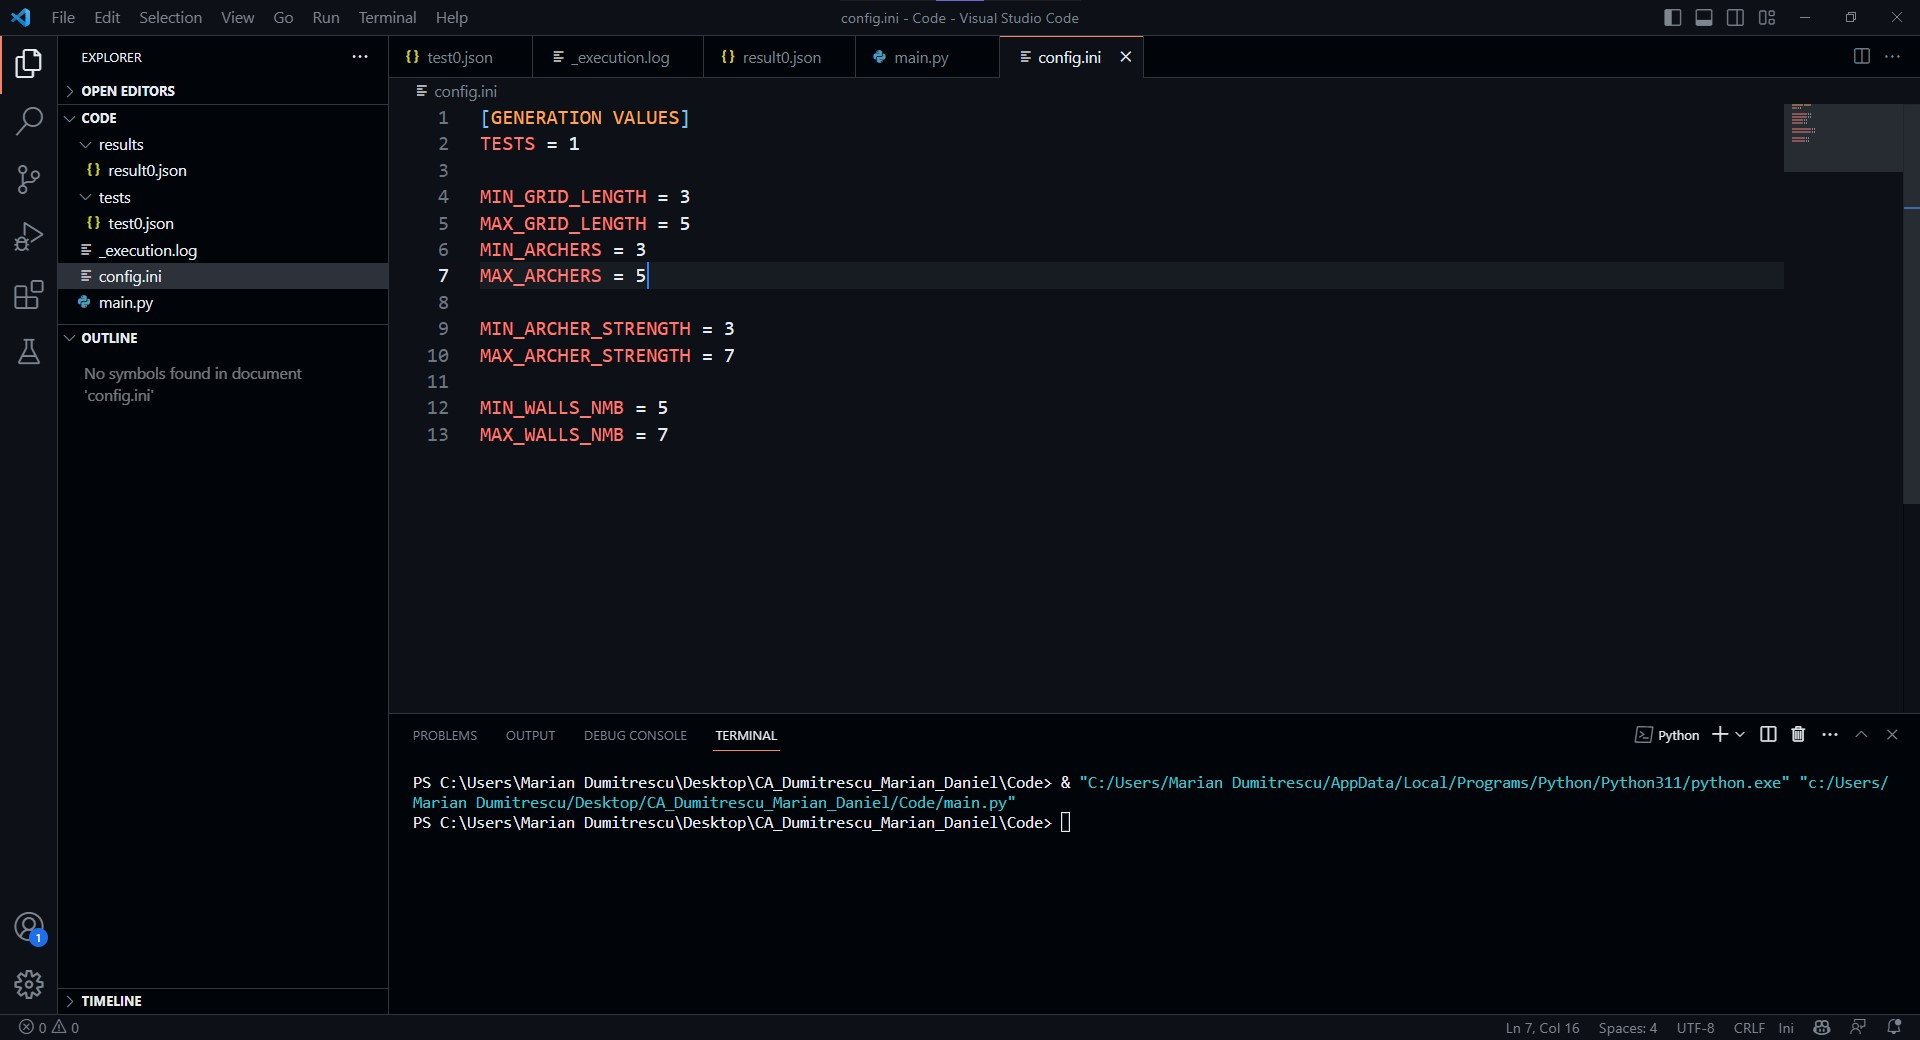
\includegraphics[width=\textwidth]{configuration.jpg}
    \vfill
    \item We will test generated values (and then export the initial values for the test) for the proposed problem and we will represent the solutions (both exported using \textit{json} file notation);\newline
    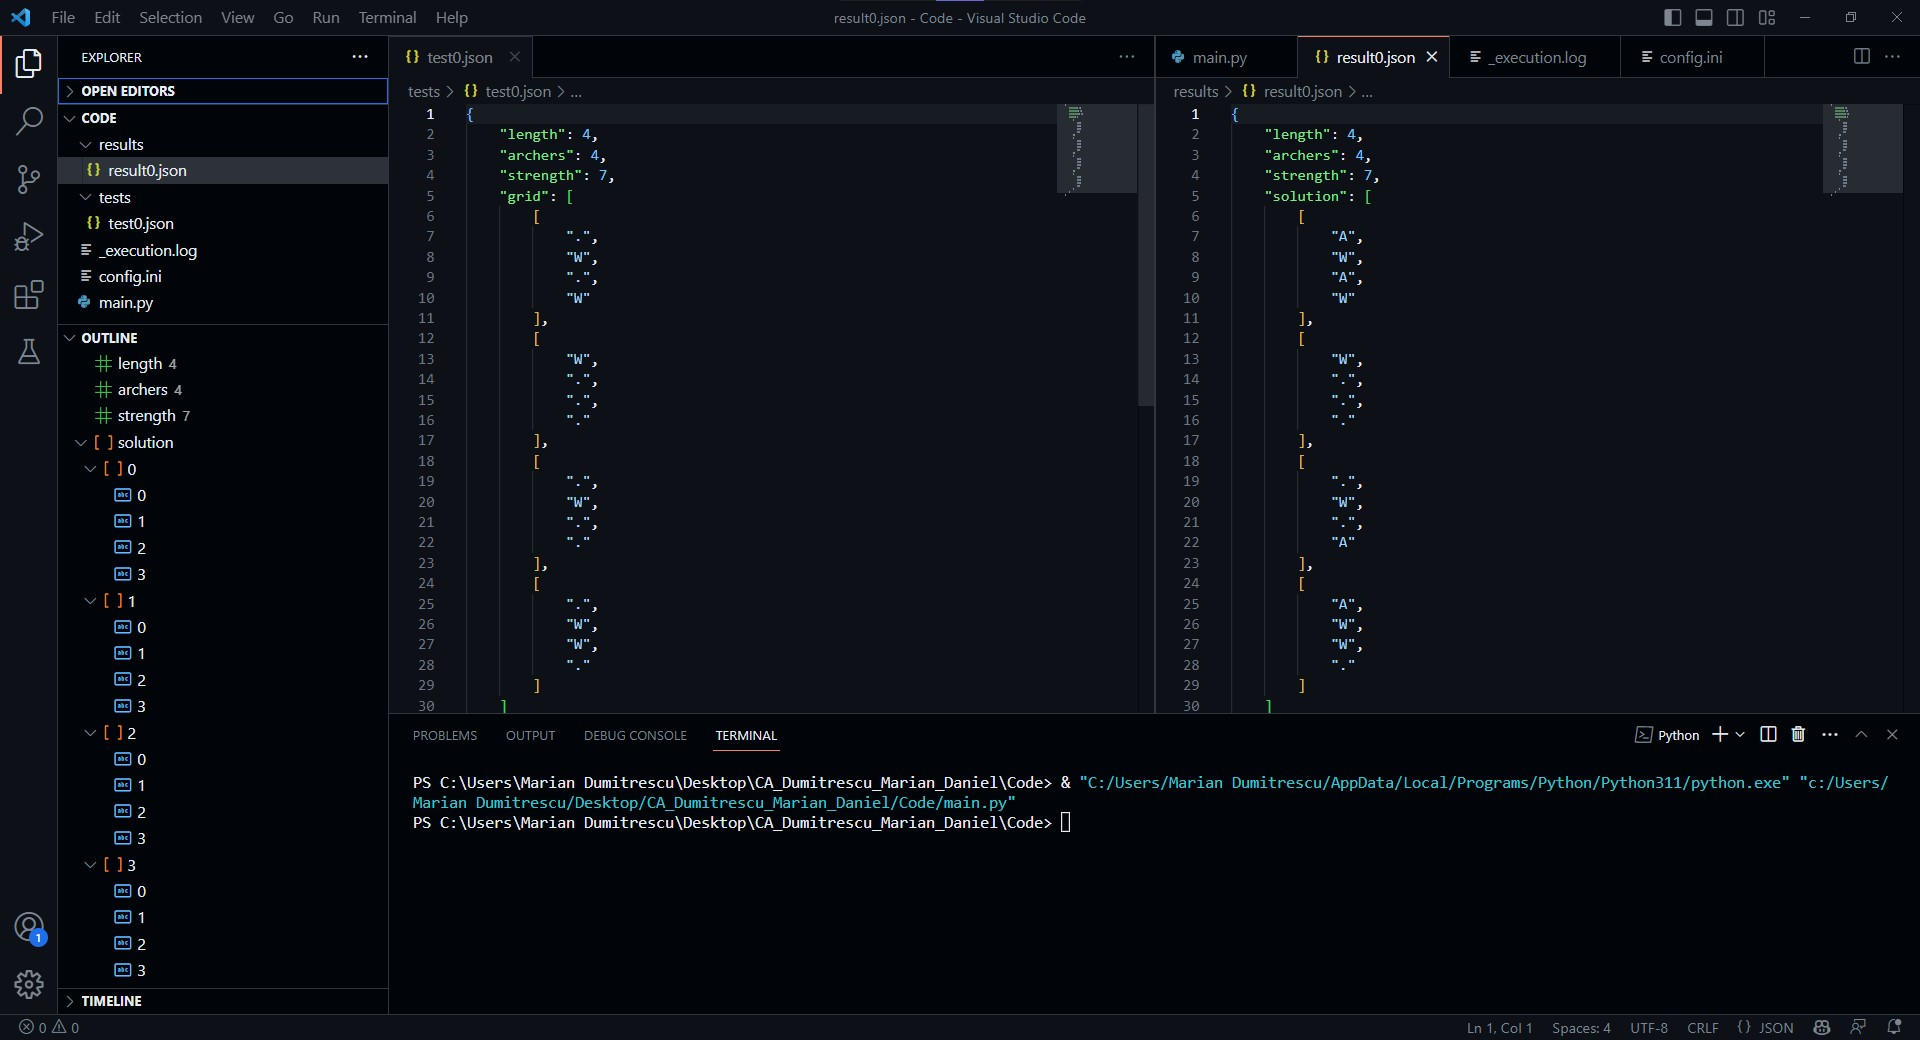
\includegraphics[width=\textwidth]{values_export.jpg}
    \item Running the proposed problem and logging our execution of the program while printing some useful visualizations for the tests and tracking the time elapsed for the said program.\newline
    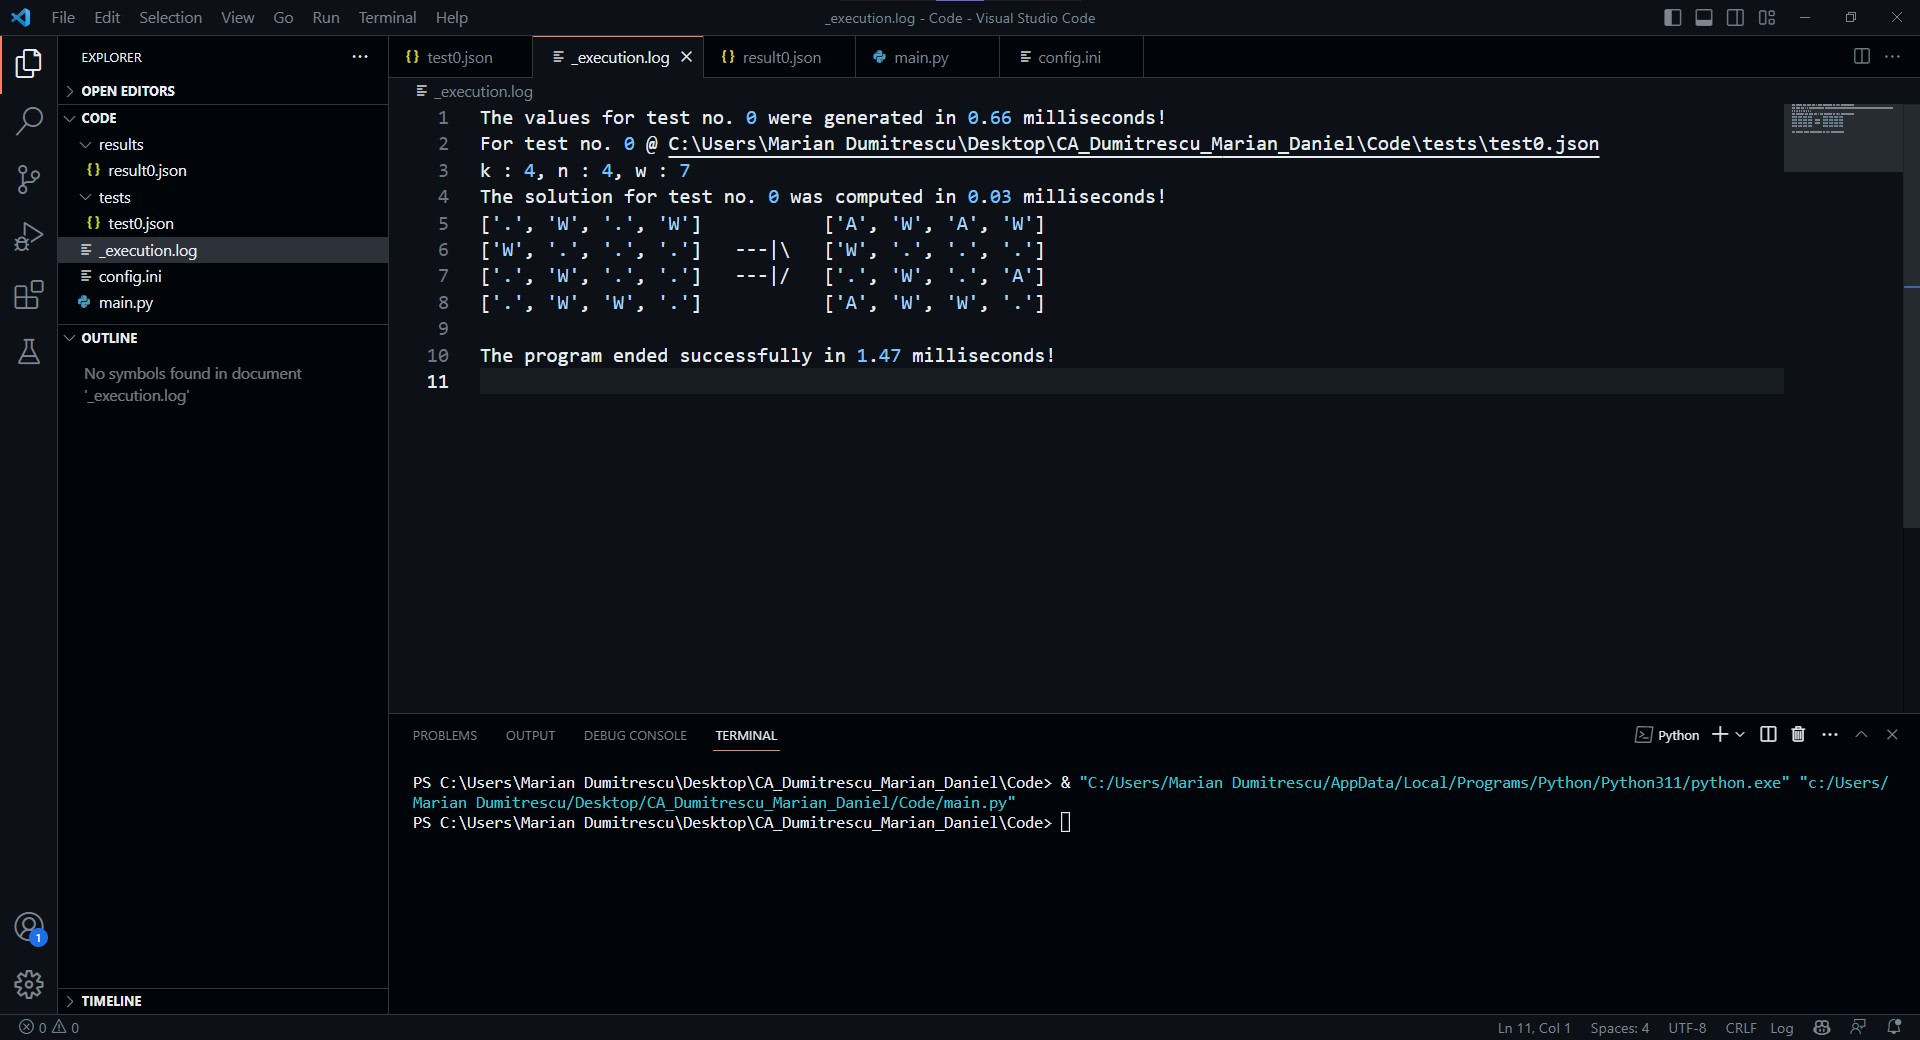
\includegraphics[width=\textwidth]{program_logging.jpg}
\vfill
\end{itemize}
The application was written in Python, because I wanted to get myself acquainted with it, thinking that it would be a great experience writing the code for the assignment while learning itself!\newline
I used the \textit{randint} function from the Python's \textit{random} module to generate the random values, \textit{configparser} module to get the configuration values for the program, Python's \textit{os} module to get some useful os-centric functions and Python's \textit{json} module to export the inputs and outputs for the program for later use, if we would like to expand the application with a Graphical User Interface in the near future.
To generate new tests, run the main.py script, and if you want to change some configuration values for the program, edit 'config.ini'.
\vfill
\section{Conclusion}
This homework assignment was a great way to learn more about uninformed search problems and a great way to learn to use the Python programming language as an important tool to define new and interesting ideas using software. I even learned a lot more about \LaTeX than last year. :)
\vfill
\section{References}
\begin{itemize}
\item \href{https://www.tablesgenerator.com/} very useful to make the examples!
\item \href{https://en.wikipedia.org/wiki/JSON}
\item \href{https://www.geeksforgeeks.org/depth-first-search-or-dfs-for-a-graph/}
\item \href{https://www.learnlatex.org/en/}
\item \href{https://www.youtube.com/} for great latex tutorials :P
\end{itemize}
\end{document}